\chapter{Estimated Timeline} 
% Main chapter title

\label{Chapter3} 
%Call reference to this chapter use \ref{ChapterX}

\lhead{Chapter 3. \emph{Estimated Timeline}} 
% Change X to a consecutive number; this is for the header on each page - perhaps a shortened title

\doublespacing
% LINE FORMATTING

\section{Estimated Timeline}
Because MTS will be developed by using prototyping model, It is estimated that the thired prototype would be stable enough to be published in the Google Play - The market of android's applications -.\linebreak \\

The second and first prototype are to find bugs and security issues in earlier time which reduce the risk and minimize the cost of fixing.\linebreak \\

Each prototype needs at least twenty-one weeks to be fully deployed. Furthermore, the work of a following prototype would be established on the nineteenth week of previous prototype. \\

\pagebreak

\subsection{Gantt Chart}

Below the Gantt Chart discripes estimated timeline for each prototype.\\

\begin{figure}[H]
	\centering
	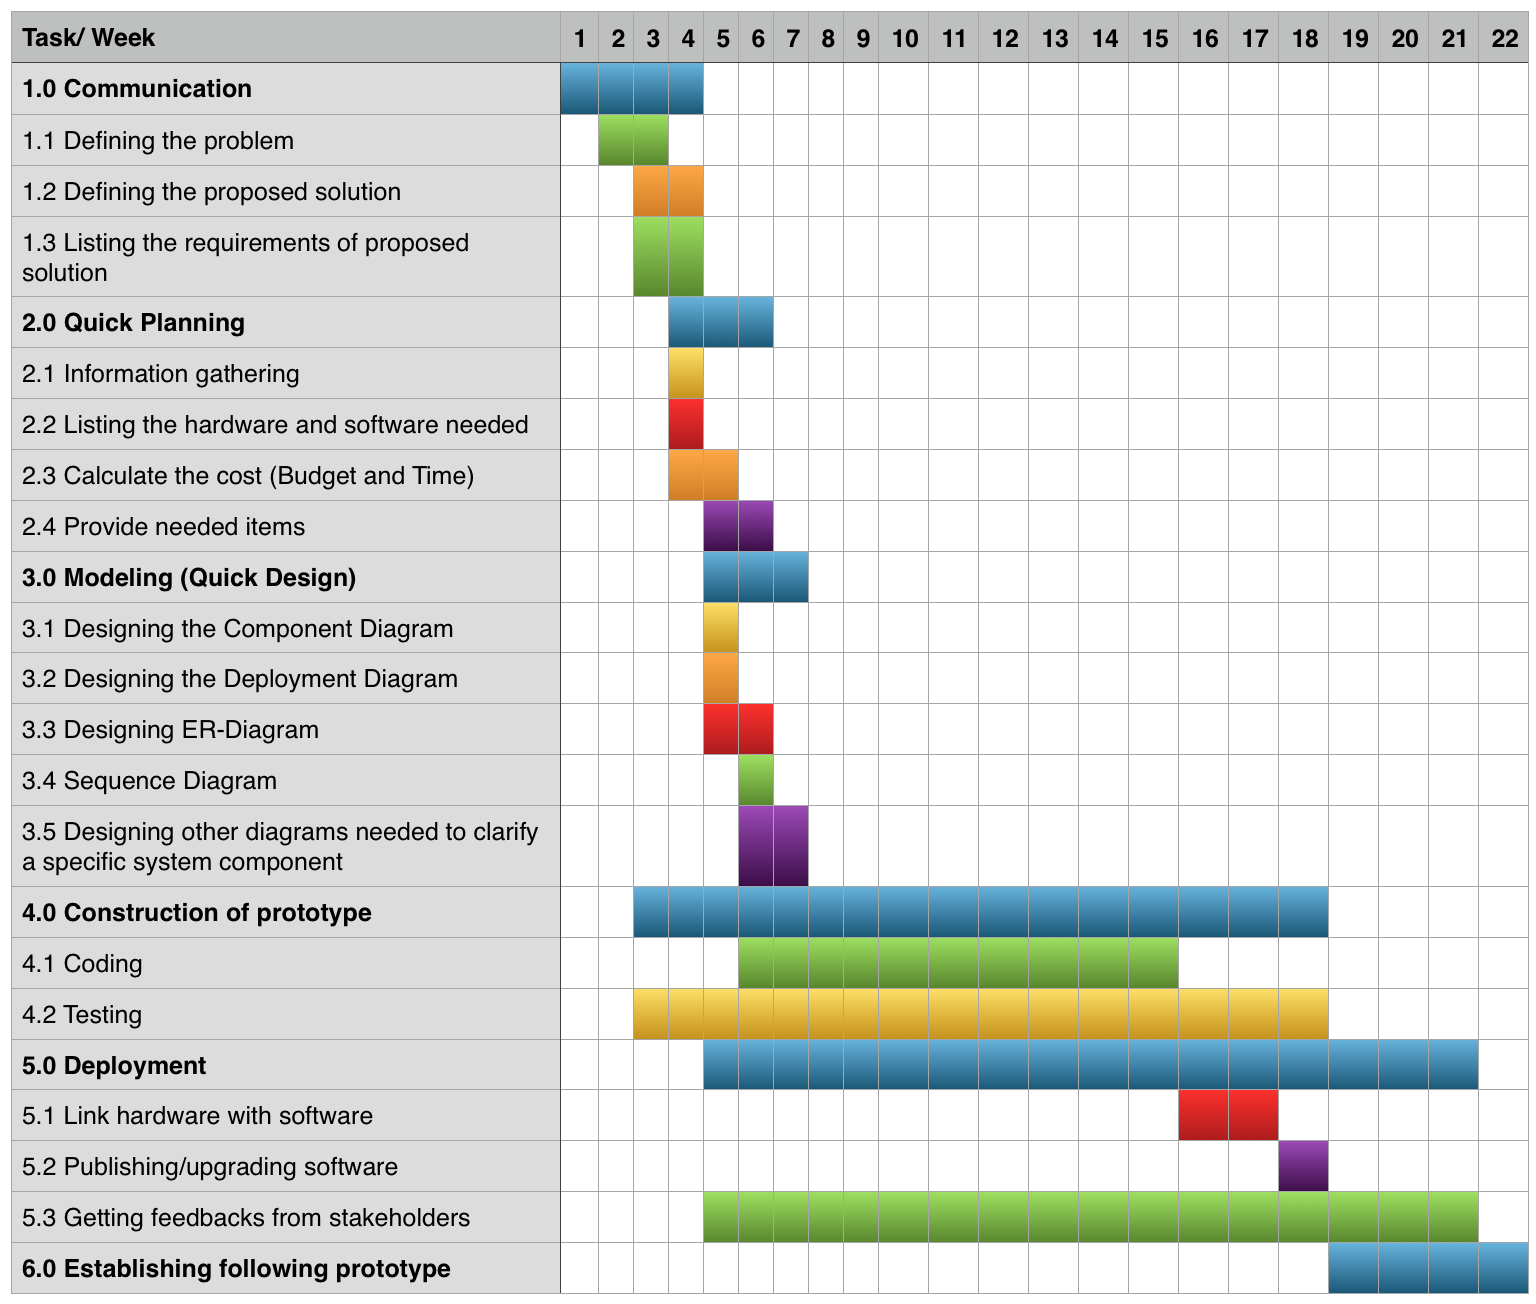
\includegraphics[scale=0.55]{Figures/FigureGanttChart.png}
	\rule{35em}{0.5pt}
	\caption[Gantt Chart: Estimated Timeline for a prototype]{Gantt Chart: Estimated Timeline for a prototype}
\end{figure}




%\clearpage
%\pagebreak

